\documentclass[11pt,border=5pt]{standalone}
\usepackage{fontspec}
\setmainfont{cmunrm.otf}[BoldFont=cmunbx.otf,ItalicFont=cmunti.otf,BoldItalicFont=cmunbi.otf]
\usepackage{amsmath}
\usepackage{unicode-math}
\setmathfont{NewCMMath-Regular.otf}
\usepackage{tikz}
\usetikzlibrary{arrows.meta,patterns,angles,quotes}
\begin{document}
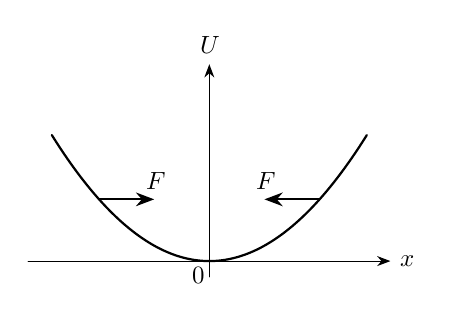
\begin{tikzpicture}[>=Stealth,font=\small,line cap=round,line join=round]
\draw[->,thin] (-2.3,0) -- (2.3,0) node[right] {$x$};
\draw[->,thin] (0,-0.2) -- (0,2.5) node[above] {$U$};
\node at (-0.14,-0.18) {$0$};
\draw[thick] plot coordinates {(-2.00000,1.60000) (-1.96667,1.54711) (-1.93333,1.49511) (-1.90000,1.44400) (-1.86667,1.39378) (-1.83333,1.34444) (-1.80000,1.29600) (-1.76667,1.24844) (-1.73333,1.20178) (-1.70000,1.15600) (-1.66667,1.11111) (-1.63333,1.06711) (-1.60000,1.02400) (-1.56667,0.98178) (-1.53333,0.94044) (-1.50000,0.90000) (-1.46667,0.86044) (-1.43333,0.82178) (-1.40000,0.78400) (-1.36667,0.74711) (-1.33333,0.71111) (-1.30000,0.67600) (-1.26667,0.64178) (-1.23333,0.60844) (-1.20000,0.57600) (-1.16667,0.54444) (-1.13333,0.51378) (-1.10000,0.48400) (-1.06667,0.45511) (-1.03333,0.42711) (-1.00000,0.40000) (-0.96667,0.37378) (-0.93333,0.34844) (-0.90000,0.32400) (-0.86667,0.30044) (-0.83333,0.27778) (-0.80000,0.25600) (-0.76667,0.23511) (-0.73333,0.21511) (-0.70000,0.19600) (-0.66667,0.17778) (-0.63333,0.16044) (-0.60000,0.14400) (-0.56667,0.12844) (-0.53333,0.11378) (-0.50000,0.10000) (-0.46667,0.08711) (-0.43333,0.07511) (-0.40000,0.06400) (-0.36667,0.05378) (-0.33333,0.04444) (-0.30000,0.03600) (-0.26667,0.02844) (-0.23333,0.02178) (-0.20000,0.01600) (-0.16667,0.01111) (-0.13333,0.00711) (-0.10000,0.00400) (-0.06667,0.00178) (-0.03333,0.00044) (0.00000,0.00000) (0.03333,0.00044) (0.06667,0.00178) (0.10000,0.00400) (0.13333,0.00711) (0.16667,0.01111) (0.20000,0.01600) (0.23333,0.02178) (0.26667,0.02844) (0.30000,0.03600) (0.33333,0.04444) (0.36667,0.05378) (0.40000,0.06400) (0.43333,0.07511) (0.46667,0.08711) (0.50000,0.10000) (0.53333,0.11378) (0.56667,0.12844) (0.60000,0.14400) (0.63333,0.16044) (0.66667,0.17778) (0.70000,0.19600) (0.73333,0.21511) (0.76667,0.23511) (0.80000,0.25600) (0.83333,0.27778) (0.86667,0.30044) (0.90000,0.32400) (0.93333,0.34844) (0.96667,0.37378) (1.00000,0.40000) (1.03333,0.42711) (1.06667,0.45511) (1.10000,0.48400) (1.13333,0.51378) (1.16667,0.54444) (1.20000,0.57600) (1.23333,0.60844) (1.26667,0.64178) (1.30000,0.67600) (1.33333,0.71111) (1.36667,0.74711) (1.40000,0.78400) (1.43333,0.82178) (1.46667,0.86044) (1.50000,0.90000) (1.53333,0.94044) (1.56667,0.98178) (1.60000,1.02400) (1.63333,1.06711) (1.66667,1.11111) (1.70000,1.15600) (1.73333,1.20178) (1.76667,1.24844) (1.80000,1.29600) (1.83333,1.34444) (1.86667,1.39378) (1.90000,1.44400) (1.93333,1.49511) (1.96667,1.54711) (2.00000,1.60000)};
\draw[->,thick] (1.4,0.784) -- (0.7,0.784) node[above] {$F$};
\draw[->,thick] (-1.4,0.784) -- (-0.7,0.784) node[above] {$F$};

\end{tikzpicture}
\end{document}
